% ~~~ [ Compilers ] ~~~~~~~~~~~~~~~~~~~~~~~~~~~~~~~~~~~~~~~~~~~~~~~~~~~~~~~~~~~~

\subsubsection{Compilers}
\label{sec:compilers}

% TODO: compiler, transpiler. compilation, transpilation. Check transpilation word.
% TODO: GHC -> Glasgow-Haskell Compiler (check acronym).

One important aspect of utilizing the IR of a compiler framework, is that the decompilation pipeline automatically gains support for transpilation (i.e. translating one programming language into another) in addition to reverse compilation. An increasing number of open source compilers (e.g. Clang, GHC, \texttt{rustc}) are capable of translating a range of source languages (e.g. C, Haskell, Rust) into LLVM IR. These compilers may be used as-is by the front-end module, thereby extending the supported source languages of the decompilation pipeline. Using this approach, the decompilation pipeline may translate $ n $ sources languages into $ m $ target languages by implementing $ n + m $ front-end and back-end modules, instead of $ n * m $ transpilers.

% TODO: Mention opt --mem2reg.

\ref{fig:front-end_source}

\begin{figure}[htbp]
	\begin{center}
		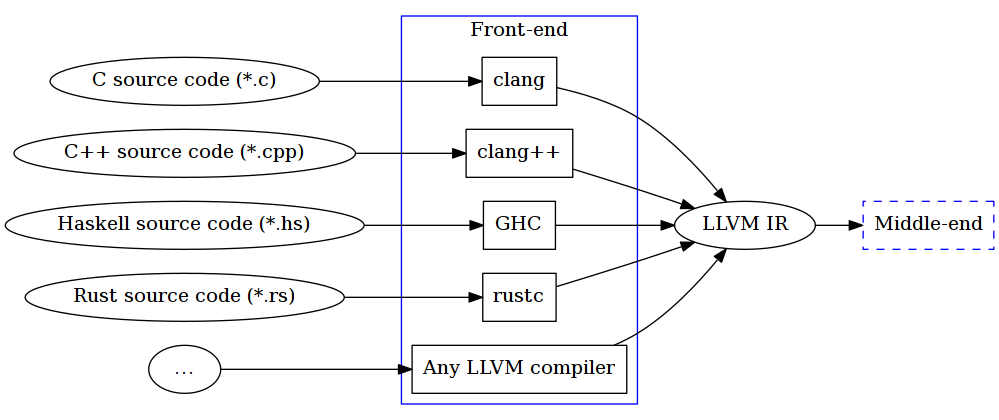
\includegraphics[width=\textwidth]{inc/front-end_source.png}
		\caption{Several open source compilers translate high-level programming languages to LLVM IR. Three such compilers are Clang, the Glasgow Haskell Compiler and the Rust compiler which translate C, Haskell and Rust respectively to LLVM IR.}
		\label{fig:front-end_source}
	\end{center}
\end{figure}
